

\lstset{
captionpos=b, 
extendedchars=true,
basicstyle=\scriptsize \sffamily, 
stringstyle=\bfseries,
frame=single,
frameround=tttt,
showstringspaces=false,
breaklines=true,
}

\lstdefinelanguage{turtle} 
{morekeywords={@prefix, a}, 
sensitive=false, 
morecomment=[l]{\#}, 
morestring=[b]",
}

% \begin{abstract}
% The FAST environment allows users to graphically compose intelligent, i.e. semantically annotated gadgets from predefined building blocks and deploy them on various mashup platforms, thus enabling the interconnection of different systems and services. Since different parties involved in the creation of gadgets and building blocks conceptualise knowledge in different ontologies, using ontology matching as a means to reconcile differences in the various conceptualisations is a crucial issue.
% This paper discusses first steps in our effort to integrate ontology matching in an end-user-oriented environment such as FAST, using an e-commerce-related scenario. We evaluate a number of tools and approaches for solving different levels of complexity in ontology matching and 
% %, which we address in this paper. We present a scenario of interconnecting e-commerce web services within a FAST gadget, the ontologies created to represent those services and the alignment tool and language used to generate and represent the ontology mappings. The testing aims firstly, to find out whether and how state-of-the-art ontology matching makes it possible to mash-up different systems and secondly, to 
% define the direction of integrating ontology matching into the FAST environment.
% 
% \keywords{Ontology Matching, User-oriented, Mashups, E-commerce}
% \end{abstract}

\section{Overview}
\label{sec:overview}

\subsection{Ontology Matching}
\label{mediation}

FAST uses ontologies to conceptualise the underlying resources used by the different components.
Ontologies embody the fundamental vehicle for conceptualising data on semantic systems; they describe the context and semantic background of data that should be known to all agents using it~\cite{gruber93towards}.
However, different ontologies are often used to describe the same domain or cover the same scenario. This is also true for FAST, where gadget building blocks can originate from different providers, who might use different ontologies to describe them. To ensure interoperability, the task of ontology matching is therefore critical in FAST.

Given two ontologies $O$ and $O'$ that need to be mapped to each other, we adopt the definition given in~\cite{shvaiko2005schema_based}: an ontology mapping element is a 5-tuple $<id, e, e', n, R>$, where 
%\begin{inparaenum}[(i)]
$id$ is a unique identifier, identifying the
mapping element, 
$e$ and $e'$ are entities (formulas, terms, classes, individuals) of the first and second ontology, respectively, 
$n$ is a confidence measure holding the correspondence value between $e$ and
$e'$, 
$R$ is the correspondence relation holding between $e$ and $e'$ (e.g., \texttt{equivalence (=)}, \texttt{more general($\sqsupseteq$)} or \texttt{disjointness($\perp$)}).
%; \texttt{overlapping($\sqcap$)}. 
%\end{inparaenum}
The alignment operation determines the mapping $M'$ for a pair of ontologies $O$ and $O'$. The alignment process can be extended by parameters, such as an input mapping, weights and thresholds and other external resources (dictionaries, thesauri, etc.). Different levels of mappings are defined:

\begin{inparaenum}[(a)]
    \item A \textit{level 0} mapping~\cite{euzenat2004api} is a set of the above mapping elements, when the entities are discreet (defined by URIs). E.g., consider the ontology $O1$ with a class \texttt{Person}, and another ontology $O2$ with a class \texttt{Human}. For this case a matching algorithm  could return the mapping element $< id_{11}, Person, Human, 0.67, = >$, meaning that the \texttt{Person} class from the first ontology is found to be equivalent to the \texttt{Human} class in the second one with a confidence measure of \texttt{0.67}.
    \item A \textit{level 1} mapping is a slight refinement of level 0, replacing pairs of elements with pairs of sets of elements.
    \item A \textit{level 2} mapping can be more complex and defines correspondences in first order logic. It uses the ontology mapping language described in~\cite{scharffe2005language}. It can describe complex correspondences, such as the one detailed in Section \ref{sub:manual_mapping}.
\end{inparaenum}
% :
% 
% \begin{equation*} \label{eq}
% \forall{x,z} grandparent(x,z) \Longrightarrow \exists{y}; parent(x,y) \wedge parent(y,z)
% \end{equation*}
 

\subsection{Ontology Matching in FAST}
\label{ominfast}

The gadget life cycle in FAST has several phases and roles associated, as detailed in \cite{hoyer-fast}. Here, we list the ones relevant for the ontology matching tasks, in decreasing order of the measure in which knowledge about ontologies is required. Note that several roles can be played by the same actor.
\begin{enumerate}[(i)]
    \item The \textit{ontology engineer} creates the ontologies used to annotate services and data. This role also includes the process of ontology matching, either automated or manually, determining if the alignment is feasible and creating so-called \emph{matching operator} building blocks, which are basic elements of the FAST screen building. The \textit{resource developer} then uses these ontologies to annotate resources created in FAST, which resources will be used by the \textit{screen developer}, who will also specify the resource type at the pre- and postconditions.
    \item Ontology matching is needed by the \textit{gadget developer} at the design-time of a screen-flow (gadget). Gadget developers use the GVS (Gadget Visual Storyboard) for building gadgets, in which they can use the matching operators to combine screens having input and output resources annotated with different ontologies. No actual matching needs to be performed in this phase, but rather the possibility of matching needs to be determined (i.e., \emph{can} two screens A and B be combined?).
%the FAST user interface determines if two resources can be combined or not (see Figure \ref{fig:screens} for a conceptual example of resources that can not be combined).
    %\item The \emph{gadget developer} combines screens to screen-flows and gadgets, and only uses ontology matching implicitly.
    \item The \textit{end-user} uses the final deployed gadget at run-time, but is unaware of the underlying resources and ontologies or the matching process. Only at run-time the actual mapping of instance data has to be performed. In this paper, we mainly consider the first two cases (i.e. ontology engineering and screen development).
\end{enumerate}


\section{Ontology Engineering Phase}
\label{sec:ontologyengineering}

\subsection{Alignment Tool}
\label{alignmenttool}

An \emph{ontology mapping} is a declarative specification of the semantic overlap between two ontologies~\cite{debruin2005wsml}. It is the result of the \emph{ontology alignment process}. This mapping is represented as a set of axioms in a \emph{mapping language}. The mapping process has three main phases:
\begin{inparaenum}[(1)]
    \item discovering the mapping (alignment phase), 
    \item representing the mapping and 
    \item exploiting the mapping.
\end{inparaenum}  

To accomplish this we need a tool to assist the ontology engineer in the ontology mapping process.
Based on the description given in Sect.~\ref{ominfast} we identify the following requirements for an alignment tool, that we will take as the basis for an ontology matching component in FAST:
\begin{inparaenum}[(i)]
\item All three phases of the process need to be accessible.
\item Matching of OWL and RDFS ontologies must be supported in the FAST project.
\item The tool should be as independent as possible, performing the alignment process with little or no user interference. This is an important requirement, since FAST is end-user oriented.
\item The tool needs to be open source, allowing it to be integrated into the free and open FAST platform.
\item The code should be suitable for porting to other languages (in particular JavaScript), allowing it to be integrated into the FAST gadget run-time.
\item It should be well documented.
\end{inparaenum}

Based on these requirements, we compared three different tools. \emph{MAFRA}~\cite{maedche2002mafra} supports an interactive and incremental process of ontology mapping. It provides an explicit notion of semantic bridges. This representation is serialisable, portable and independent from the mapped languages. The bridges, however, have been designed to be used within the MAFRA system, and the alignment process needs to be done through the provided GUI. \emph{RDFT}~\cite{omelayenko2002rdft} is a small language originally designed to map between XML and RDF. The results are mappings represented in DAML+OIL, that can be executed in a transformation process. No hints are given to add alignment methods or extending the format and the tool does not longer seem to be available. \emph{Alignment API}~\cite{euzenat2004api} is the tool best matching our requirements, satisfying all the desired conditions. It is still under active development, provides an API and its implementation, is open source (GPLv2 or above) and written in Java, providing an easy way to embed it into other programs. Alignment API can be extended by other representations and matching algorithms, it can be invoked through the command line interface (thus working without user interference) or one of the two available GUI implementations, or it can be exposed as an HTTP server. The tool allows for testing different alignment methods and can generate evaluation results based on a reference alignment. Alignment API can generate the mapping results in XSLT, therefore providing an easy way to integrate them into other systems.

\subsection{Scenario Description}
\label{scenario}

In our evaluation scenario, which is taken from the e-commerce domain, a user needs to build a gadget which combines data from major e-commerce services, allowing to aggregate item lists from all of them in a combined interface.
As examples in our scenario, we consider the two most popular online shopping websites\footnote{\url{http://alexa.com/topsites/category/Top/Shopping}, checked 01/11/2009}, Amazon and eBay, along with the BestBuy site. The latter is an interesting case, because it exposes its data in RDF using the GoodRelations (GR) ontology~\cite{hepp-goodrelations}, which has recently gained a lot of popularity. It is therefore one of the first major e-commerce sites to provide semantic metadata.

\begin{figure}
    \centering
        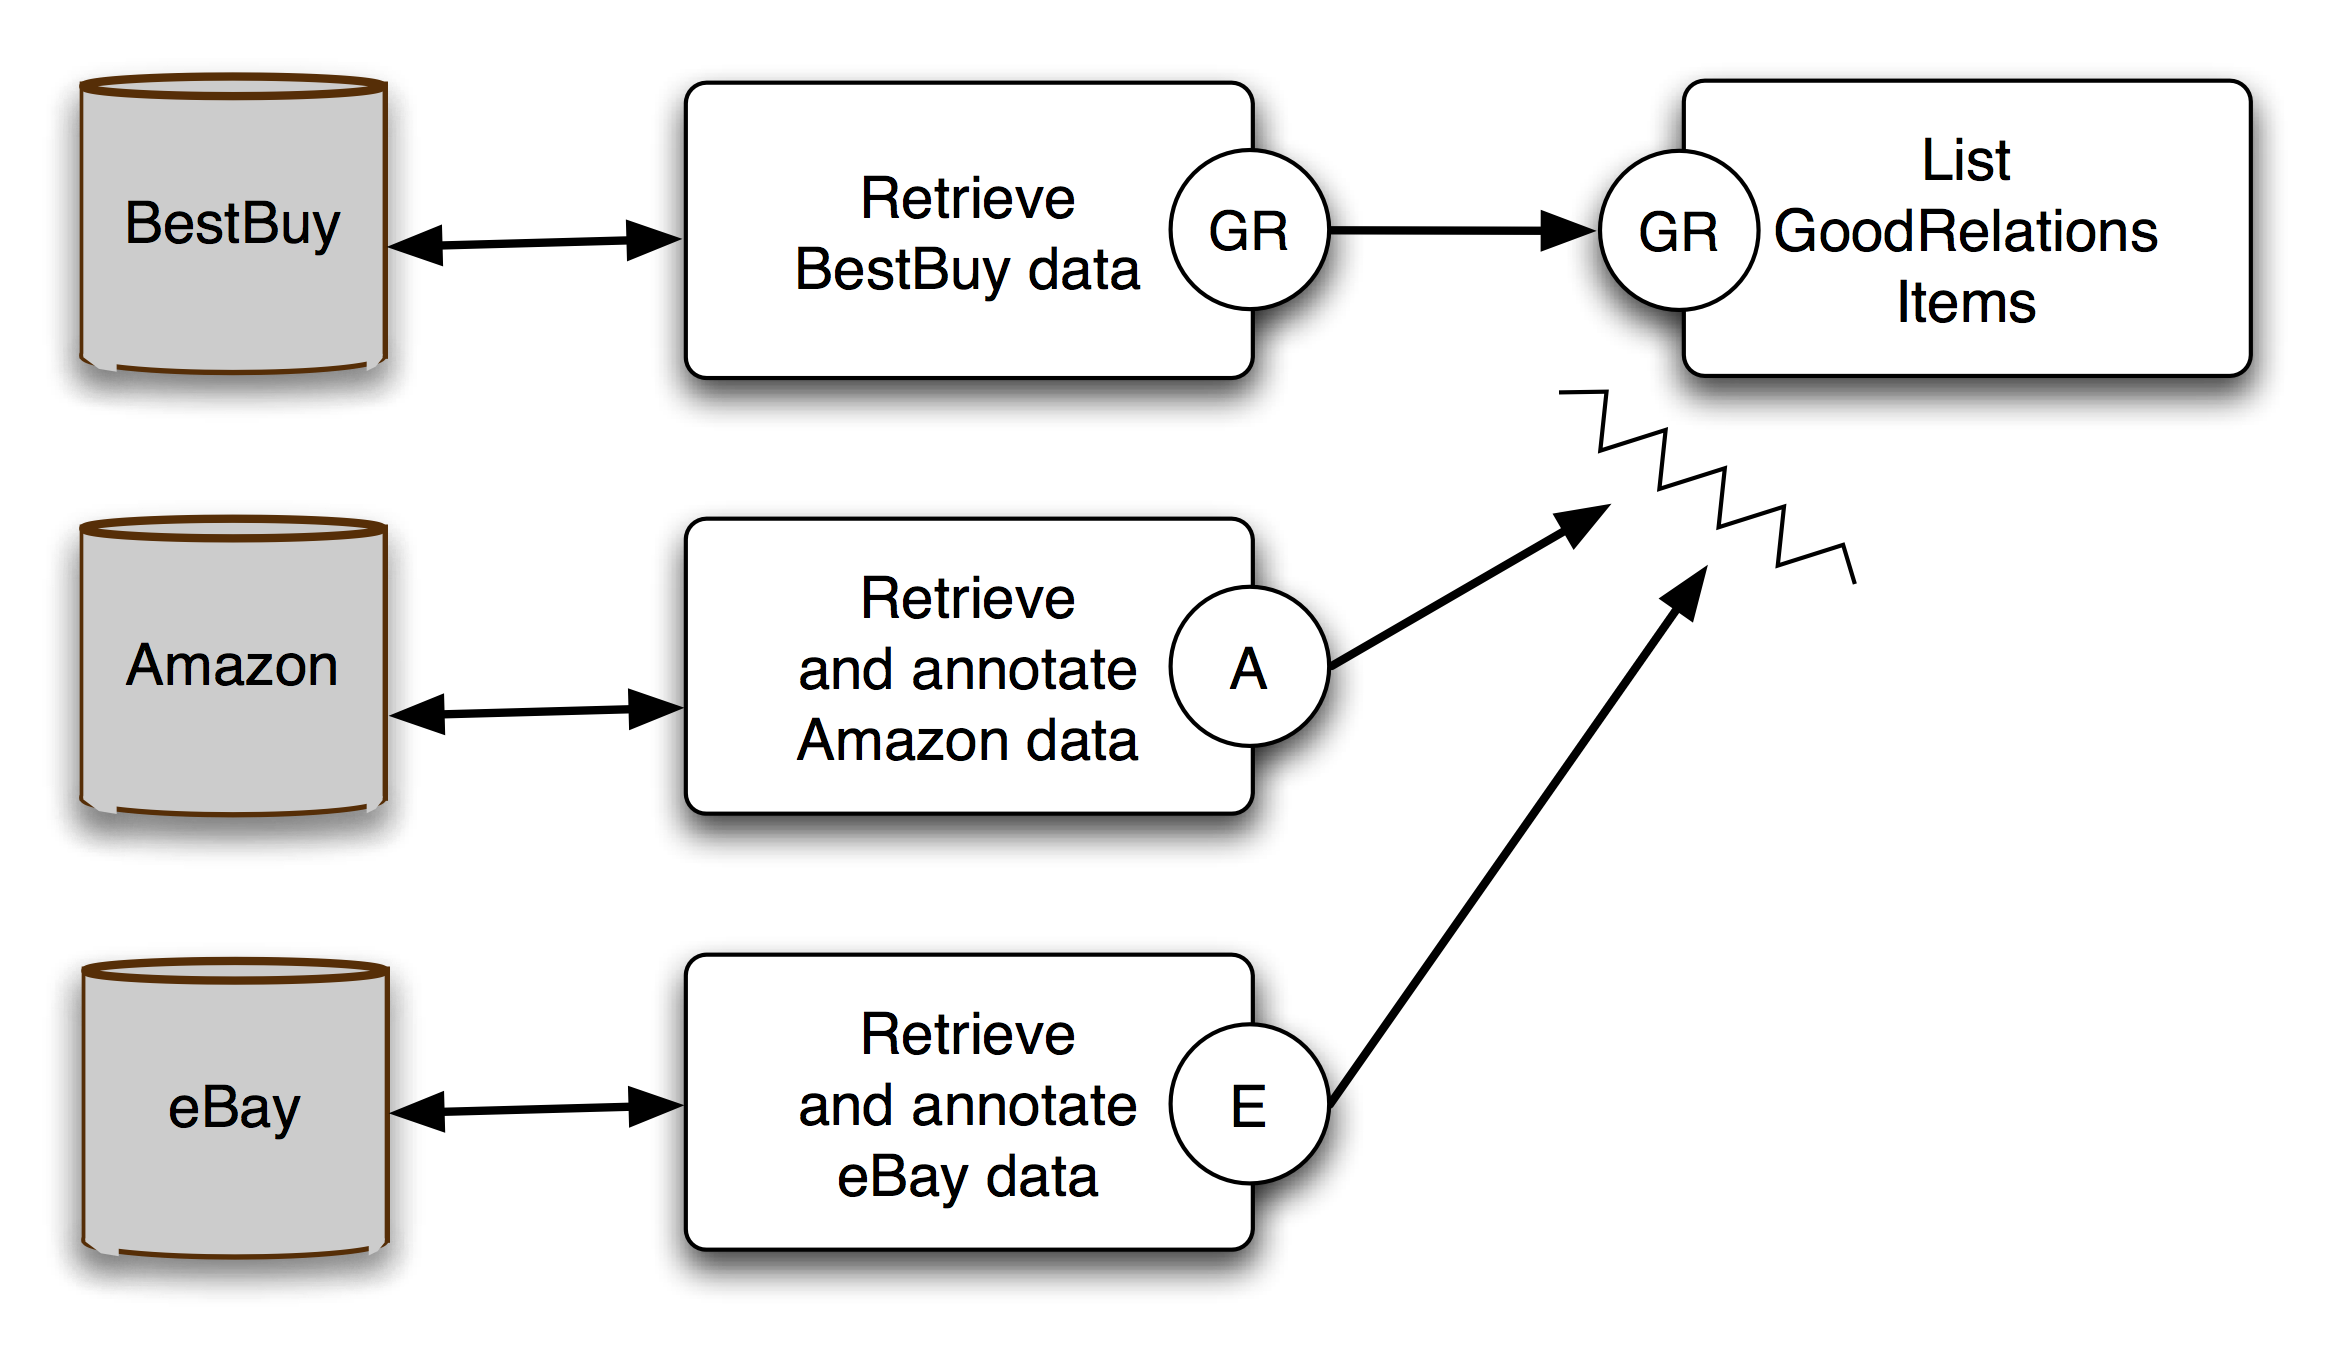
\includegraphics[width=8cm]{images/screens_diagram.png}%[bb=0 0 201 126]
        \caption{Three gadget components retrieving incompatible data}
    \label{fig:screens}
\end{figure}

Figure~\ref{fig:screens} illustrates our scenario. There are three retrieval components that wrap the different e-commerce sites and provide data according to three different ontologies: the GR ontology, the Amazon ontology (A) and the eBay ontology (E). Another component displays GR items for display to the user, but not A or E items. If the gadget designer wants to aggregate data from all three services in the display, there will therefore have to be a mapping present between A and E on the one hand, and GR on the other.

%, say we have a component that accesses the BestBuy service and retrieves RDF data that uses the GoodRelations ontology. In other words, the output of this component is GoodRelations data. Another component takes this data and displays them in a list, i.e. this component only accepts GoodRelations data for display. Since both components use the same ontology, they can be combined. However, now suppose we have two additional components, which access the Amazon and eBay services and retrieve items from there, which are then represented using the Amazon and eBay ontologies, respecitvely. The user wants to list items from all three sources in the same display component. However, since all three ontologies are incompatible, this is not possible out of the box. What is necessary is a mapping between the Amazon and GoodRelations, as well as eBay and GoodRelations ontologies.

%We have thus a case, where we want to aggregate data using three different ontologies, so aligning them to a common ontology is the only possible solution.

\subsection{Ontologies}
\label{ontologies}
Of the three ontologies used in our evaluation, only GoodRelations is a real-world, extensive ontology for e-commerce. The other two, i.e., the Amazon and the eBay ontologies were developed for simulation purposes as simplified versions of what would be used in the real-life scenarios. They were designed to showcase particular features of ontology mapping in our scenario.

\paragraph{GoodRelations:}
This ontology is aimed at annotating so-called ``offerings'' on the Web, which can be products or services. The ontology features support for ranges of units, measurements, currencies,  shipping and payments, common business functions (sell, lease, repair, etc.) and international standards (ISO 4217 or UNSPSC) and codes (e.g., EAN or UPC) in the field.
The main class is \texttt{Offering},
which represents an announcement by a \texttt{BusinessEntity} to provide a \texttt{ProductOrService} with a given \texttt{BusinessFunction}. It may be constrained in terms of eligible business partner, countries, quantities, and other properties. It is also described by a given \texttt{PriceSpecification}. The super-class for all classes describing products or service types is \texttt{ProductOrService}. This top-level concept has sub-classes representing actual product instances, product models and dummy product placeholders. A product is described by its title and description, manufacturer, make and model, etc. 
% While GoodRelations offers terminology to allow a much higher expressivity, we will restrict the discussion to those terms relevant for our scenario.


% \begin{center}
% \lstset{captionpos=b, breaklines=true}
% \lstset{frame=single, basicstyle=\scriptsize}
% \lstset{caption=Basic GoodRelations data in N3 notation, label=listing_gr}
% \lstset{language=XML}
% \begin{lstlisting}
% :Offering_8794691     a gr:Offering;
%   gr:hasPriceSpecification 
%       :UnitPriceSpecification_8794691_1;
%   gr:includesObject :TypeAndQuantityNode_8794691_1;
% 
% :UnitPriceSpecification_8794691_1     a gr:UnitPriceSpecification;
%   gr:hasCurrency "USD"^^xsd:string;
%   gr:hasCurrencyValue "749.99"^^xsd:float;
%   gr:hasUnitOfMeasurement "C62"^^xsd:string;
% 
% :TypeAndQuantityNode_8794691_1     a gr:TypeAndQuantityNode;
%   gr:amountOfThisGood "1.0"^^xsd:float;
%   gr:hasUnitOfMeasurement "C62"^^xsd:string;
%   gr:typeOfGood :ProductOrServicesSomeInstancesPlaceholder_8794691 .
% 
% :ProductOrServicesSomeInstancesPlaceholder_8794691 a gr:ProductOrServicesSomeInstancesPlaceholder;
%   gr:hasEAN_UCC-13 "0013803096095"^^xsd:string;
%   gr:hasMakeAndModel :PoSM_8794691;
%   rdfs:comment "With Auto Optimization and [...]"@en;
% 
% :PoSM_8794691     a gr:ProductOrServiceModel;
%   gr:hasManufacturer <bbuy:Manufacturer_Canon>;
%   rdfs:label "Canon EOS Digital Rebel [...]"@en;
%   rdfs:comment "With Auto Optimization and [...]"@en;
% \end{lstlisting}
% \end{center}


\paragraph{Amazon Ontology:}
We have created a small Amazon ontology based on a subset of the datatypes supported by the web service exposed by Amazon to third-party agents. The ontology describes \texttt{Items} based on the \texttt{ItemAttributes} description given in the Amazon Product Advertising API documentation\footnote{\url{http://docs.amazonwebservices.com/AWSECommerceService/latest/DG/}}.
The ontology features three classes for describing a product. Example instance data is given in List.~\ref{listing_amazon}.
\begin{inparaenum}[(1)]
    \item \texttt{Item} represents an Amazon item, defined by a title, a manufacturer, a product group (DVD, Book, etc.), an international EAN code, an ASIN (unique Amazon id), an author (for books) and a \texttt{ListPrice}. 
    \item \texttt{Company}, described by a  legal name, is used for representing the manufacturer of an \texttt{Item}.
    \item \texttt{ListPrice} has two properties: \texttt{hasCurrencyCode}, representing an ISO 4217 currency code (e.g. GBP or EUR), and \texttt{hasAmount} representing the price in the given currency.
\end{inparaenum}


% \begin{figure}[ht]
\lstset{caption=Simplified Amazon ontology data in N3 notation, label=listing_amazon}
\lstset{language=turtle}
\begin{lstlisting}
:Item_7590645 a amzn:Item;
   amzn:hasASIN "B0012YA85A";
   amzn:hasManufacturer :Manufacturer_Canon;
   amzn:hasModel "XSI Kit";
   amzn:hasPrice :Price_7590645_1;
   amzn:hasProductGroup "Electronics";
   amzn:hasTitle "Canon Digital Rebel XSi [...]" .
:Manufacturer_Canon a amzn:Company;
   amzn:hasLegalName "Canon" .
:Price_7590645_1 a amzn:ListPrice;
   amzn:hasAmount "575.55";
   amzn:hasCurrencyCode "GBP" .
\end{lstlisting}
% \end{figure}

\paragraph{eBay Ontology:}
The eBay ontology was created based on the eBay Shopping API\footnote{\url{http://developer.ebay.com/DevZone/shopping/docs/CallRef/index.html}} and is supposed to annotate data retrieved through the web service described by the API.
% \begin{center}
% \lstset{captionpos=b, breaklines=true}
% \lstset{frame=single, basicstyle=\small}
% \lstset{caption=Simplified eBay ontology data in N3 notation, label=listing_ebay}
% \lstset{language=XML}
% \begin{lstlisting}
% 
% :SimpleItem_1320648     a ebay:SimpleItem;
%   ebay:hasItemID "E012Y090912";
%   ebay:hasBidCount :"4";
%   ebay:hasCountry "UK";
%   ebay:hasCurrentPrice :Price_1320648_1;
%   ebay:hasPrimaryCategoryName "Electronics";
%   ebay:hasTitle "Canon Digital Rebel XSi [...]" .
%   ebay:hasDescription "Camera is practically unused. It's like new."
% 
% :Price_1320648_1     a ebay:CurrentPrice;
%   ebay:hasAmount "575.55";
%   ebay:hasAmountType "GBP" 
% \end{lstlisting}
% \end{center}
The ontology features three basic classes,
%  (see Listing \ref{listing_ebay} for an example of ebay data)
\begin{inparaenum}[(1)]
    \item \texttt{SimpleItem} represents an eBay \texttt{Item}, that is sold by a \texttt{SimpleUser}. It is described by a title, a \texttt{CurrentPrice} (specifying the highest bid, or the selling price of fix-priced items), primary category name, manufacturer, model, EAN code, item ID (a unique eBay ID), bid count, end time of bid, country where the item is located, and a product ID (which supports major international product codes --- this property is from the Finding API).
    \item The \texttt{CurrentPrice} features a \texttt{hasAmountType} property, specifying the currency code, and a \texttt{hasAmount} property, which is the amount of money for a price per unit.
    \item \texttt{SimpleUser} contains information about eBay users. Users are described by a user ID, about me URL and the seller's positive feedback score. This class will not be used for capturing information on goods for our scenario, but is an essential component of the eBay system, which was the reason for its inclusion in the ontology.
\end{inparaenum}

\subsection{Testing and Results}
\label{testing}

We present the approach an ontology engineer has to take to discover and represent ontology mappings, and a means to exploit them after the they have been discovered and appropriately represented.

There is a major paradigm difference between the GoodRelations ontology and the other two ontologies (see Sect.~\ref{sub:manual_mapping} for details). After some initial testing, we concluded that automatic mapping from GR to A/E using the string-based methods employed by the Alignment API tool was not feasible. Therefore, the following sections report on \emph{automatic mapping} for the A--E pair --- which are similar enough to be suitable for level 0 mapping ---, and \emph{manual mapping} for the GR--A/E pairs.

\subsubsection{Automatic Mapping}

% \paragraph{The Matcher} % (fold)
% \label{par:the_matcher}

% paragraph the_matcher (end)
For automatic mapping of level 0 mappings, we used a simple string distance-based algorithm provided by Alignment API~\cite{euzenat2004api}, which computes the string distance between the names of the entities to find correspondences between them. Four methods have been used for computing the distance:
\begin{inparaenum}[(1)]
    \item equality, which tests whether the names are identical, 
    \item Levenshtein distance (number of character operations needed), 
    \item SMOA distance (which is a specialised distance for matching ontology identifiers) and
    \item a Wordnet-based~\cite{fellbaum1998wordnet} distance using the JWNL library with Wordnet.
\end{inparaenum}

The alignment description derived from these methods is given based on a simple vocabulary, containing a pair of ontologies and a set of correspondences, which express relations between entities of the two ontologies.
We used the level 0 mapping representation for representing simple mappings, which map discrete entities of the two ontologies. Thus the representation of the correspondences is given with the five elements described (with the \texttt{id} being optional), as shown in List.~\ref{listing_correspondence}. Similar mappings were were also used for more complex, manually-created representations (level 2), as detailed in Sect.~\ref{sub:manual_mapping}.

% \begin{figure}[ht]
% \begin{minipage}{\linewidth}
\lstset{caption=Level 0 mapping element example, label=listing_correspondence}
\lstset{language=turtle}
\begin{lstlisting}
<level_0_mapping> a align:Cell;
  align:entity1 amzn:hasCurrencyCode;
  align:entity2 ebay:hasAmountType;
  align:measure "1.0"^^xsd:float;
  align:relation "=" .
\end{lstlisting}
% \end{minipage}
% \end{figure}

% \subsubsection{Using the Tool.}
% The Alignment API tool can be used through a GUI, as a server or from the
% command-line interface, of which we have chosen the last one.
% The tool reads two RDF/OWL ontologies, computes the alignment between them, 
% performs some thresholding and displays the results. It can render the output
% in a number of formats, including HTML and XSLT.
% 
% An additional feature of the tool is its ability to evaluate results based on
% a reference alignment, and output the evaluation results in a table,
% or plot them as \LaTeX{} graphs.

\paragraph{Testing Procedure}
For the Amazon--eBay pair we set up a reference alignment, against which the results are evaluated.
We then ran the matching process for all for methods:
\begin{inparaenum}[(1)]
    \item equality,
    \item Levenshtein distance with a confidence threshold of \texttt{0.33} (meaning that any correspondence having a smaller confidence measure will be excluded),
    \item SMOA distance with a threshold of \texttt{0.5} and
    \item Wordnet distance using a threshold of \texttt{0.5}.
\end{inparaenum}
To apply the results, we rendered an XSLT template to transform an example dataset.

\paragraph{Results}

The results of automatically aligning the Amazon and eBay ontologies were quite favourable. As shown in Tab.~\ref{table_results}, we captured the four main parameters used in information retrieval, as described in \cite{olson2008advanced}. These four parameters are used for evaluating the performance of the alignment methods: 
\begin{inparaenum}[(1)]
    \item \textit{Precision}, the fraction of results that are correct --- the higher, the better, 
    \item \textit{Recall}, the ratio of the correct results to the total number of correct correspondences --- the higher, the better, 
    \item \emph{Fallout}, the fraction of incorrect results - the lower the better, and 
    \item \emph{F-measure}, which measures the overall effectiveness of the retrieval by a harmonic mean of precision and recall --- the higher, the better.
\end{inparaenum}

\begin{table}
    \centering
    \caption{Alignment results: Precision, Recall, Fallout and F-Measure}
    \label{table_results}

    \begin{tabular}{rrrrr}
        \toprule
        & \textbf{precision} & \textbf{recall} & \textbf{fallout} & \textbf{f-measure}\\
        \midrule
        \textbf{reference} & 1.00 & 1.00 & 0.00 & 1.00\\
        \textbf{equality} & 1.00 & 0.38 & 0.00 & 0.55\\
        \textbf{SMOA} & 0.43 & 0.75 & 0.57 & 0.55\\
        \textbf{Levenshtein} & 0.40 & 0.75 & 0.60 & 0.52\\
        \textbf{JWNL} & 0.67 & 0.75 & 0.33 & 0.71\\
        \bottomrule
    \end{tabular}
\end{table}

The first row (reference) shows the reference alignment, which, naturally, has both perfect precision and recall. We can observe what intuition has predicted, namely that pure string equality (equality) is far too simple and irrelevant, by only taking identical labels. By using string distances and giving certain thresholds (Levenshtein and SMOA), we can see that the results are much less precise, but have a better recall, since this allows for entities having similar names to be discovered, at the expense of having quite a few incorrect results (lower precision); the thresholds allow for low-scored cases to be eliminated, although this results in the exclusion of some correct correspondences. The last column (JWNL) contains the results of the Wordnet-enabled method, which shows quite an improvement (precision of 0.67 and a recall of 0.75), due to the lexical analysis, which performs a much more relevant comparison of strings, giving a high number of correct results. The precision of the JWNL alignment shows only a tiny drop below the recall value, meaning that the number of incorrect correspondences discovered is small, and the main source of error is from the number of correspondences not discovered.


% \begin{center}
% \begin{figure}
% %% Plot generated by GenPlot of alignapi
% \begin{center}
% \begin{tikzpicture}[cap=round, scale=0.75]
% % Draw grid
% \draw[step=1cm,very thin,color=gray] (-0.2,-0.2) grid (10.0,9.0);
% \draw[|-|] (-0,0) -- (10,0);
% %\draw[dashed,very thin] (0,0) -- (5,8.66) -- (10,0);
% \draw[dashed,very thin] (10,0) arc (0:60:10cm);
% \draw[dashed,very thin] (0,0) arc (180:120:10cm);
% \draw (0,-0.3) node {$precision$};
% \draw (10,-0.3) node {$recall$};
% % Plots
% \draw plot[mark=+,] coordinates {(5.0,8.660254037844386)};
% \draw (5.01,8.370254037844385) node[anchor=south west] {Reference};
% \draw plot[mark=+,] coordinates {(9.296875,3.6834922606644636)};
% \draw (9.306875,3.3934922606644633) node[anchor=south west] {Equal};
% \draw plot[mark=+,] coordinates {(3.1058673469387754,2.9531229168449795)};
% \draw (3.115867346938775,2.6631229168449793) node[anchor=south west] {SMOA0.5};
% \draw plot[mark=+,] coordinates {(2.9875000000000003,2.6598578439458005)};
% \draw (2.9975,2.3698578439458003) node[anchor=south west] {Levenshtein0.33};
% \draw plot[mark=+,] coordinates {(4.409722222222222,4.99987943527481)};
% \draw (4.419722222222222,4.70987943527481) node[anchor=south west] {JWNL};
% 
% \end{tikzpicture}
% \end{center}
% \caption{Comparison of the four methods, against the reference alignment,\newline
% showing the distances from 0 precision and 0 recall}
% \label{fig:figure_alignment}
% \end{figure}
% \end{center}



We can deduce that the results provided are satisfactory, even though the methods used were simple, string-based ones, and the process was completely automated without any user input.
We are therefore confident that through some user assistance or an initial input alignment the tool can achieve 100\% correct results.


% \paragraph{XSLT:}
% One of the appealing features of the Alignment API is that it can render the results in XSLT, thus specifying a set of rules which make it possible to transform an  XML file from one format to the other. We have generated such an XML transformation description, and with the simple Linux application \texttt{xsltproc} (run from the command line) we have managed to transform data (limited, of course by the incompleteness of the alignment) from the Amazon ontology into data annotated by the eBay vocabulary. 
%Please refer to Appendix A for a listing of an example transformation.

\subsubsection{Manual Mapping} % (fold)
\label{sub:manual_mapping}

The GoodRelations ontology employs a unique paradigm, different from the paradigms of Amazon and eBay. In GR everything is centred around an instance of \texttt{Offering} and a graph of other instances attached to it, whereas for Amazon (and similarly for eBay), the main class is \texttt{Item}, which holds all relevant properties. In principle, \texttt{Item} would correspond to \texttt{ProductOrService} in GoodRelations, but the properties of the \texttt{Item} class are reflected as properties of many different classes in GR. 

Though the infeasibility of automating this alignment became obvious, we have represented the alignment in the mapping language supported by the tool, as a level 2 mapping (described in Sect. \ref{mediation}).
 % (the mapping has been created between Amazon and GoodRelations, since the eBay and Amazon ontologies are very similar in approach, and mapping eBay to GoodRelations would be an indentical task). 
This mapping description can later be used by the run-time gadget code. List.~\ref{listing_gr_a} shows an example mapping between two properties of the two ontologies, specifying that the relationship is \texttt{Equivalence} with a certainty degree of \texttt{1.0}. This fragment does not show, but assumes the equivalence correspondence between the classes \texttt{Item} and \texttt{Offering}, which is a trivial level 0 mapping. This mapping specifies the relation

\begin{equation*} \label{eq}
\begin{split}
\forall{v,z}; hasEAN(v,z) & \Longrightarrow \exists{x, y}; includesObject(v,x) \wedge \\
&typeOfGood(x,y) \wedge hasEAN\_UCC\_13(y,z),
\end{split}
\end{equation*}

meaning that the \texttt{hasEAN} property of \texttt{v} in the Amazon ontology corresponds to the \texttt{hasEAN\_UCC\_13} property of the \texttt{typeOfGood} of the \texttt{includesObject} of \texttt{v} in GoodRelations. The domains and ranges of the properties are inferred, thus it is deduced, that in \texttt{Amazon v} is of type \texttt{Item} and \texttt{z} is \texttt{int}, and in \texttt{GoodRelations v, x, y} and \texttt{z} are instances of the classes \texttt{Offering}, \texttt{TypeAndQuantityNode}, \texttt{ProductOrService} and \texttt{int}, respectively.

\begin{figure}[ht]
\lstset{caption=Fragment of the Amazon--GoodRelations mapping, label=listing_gr_a}
\lstset{language=turtle}
\begin{lstlisting}
<level_2_mapping> a align:Cell;
   align:entity1 amzn:hasEAN;
   align:entity2 
      [ a align:Property;
        align:first gr:includesObject;
        align:next gr:hasEAN_UCC_13,
           gr:typeOfGood ];
     align:measure "1.0"^^xsd:float;
     align:relation "Equivalence" .

amzn:hasEAN a align:Property .
gr:hasEAN_UCC_13 a align:Property .
gr:includesObject a align:Relation .
gr:typeOfGood a align:Relation .
\end{lstlisting}
\end{figure}

% \begin{center}
% \lstset{caption=Fragment of the Amazon--GoodRelations mapping, label=listing_gr_a}
% \lstset{language=xml}
% \begin{lstlisting}
% <Cell rdf:about="MappingRule_01">
%  <entity1><omwg:Property rdf:about="&amzn;hasEAN"/></entity1>
%  <entity2>
%   <omwg:Property>
%     <first><Relation rdf:about="&gr;includesObject"/></first>
%     <next><Relation rdf:about="&gr;typeOfGood"/></next>
%     <next><Property rdf:about="&gr;hasEAN_UCC_13"/></next>
%   </omwg:Property>
%  </entity2>
%  <measure rdf:datatype="&xsd;float">1.0</measure>
%  <relation>Equivalence</relation>
% </Cell>
% \end{lstlisting}
% \end{center}

Using this representation, complex correspondences can be modelled, using first order logic constructs.

\subsection{Service Wrapping Tool}
\textbf{\textit{Kassel will describe the service wrapping tool they've developed, that creates mapping instances between ontologies. 
A description of the front-end and the creation of the mapping rules will be given here.}}

\subsection{Creating the Operator}

\textbf{\textit{Kassel will describe the creation of the matching operator in the catalogue and the storage of the mapping rules.}}

\section{Gadget Building Phase}
\label{sec:gadgetbuilding}
Every time ontology matching is performed and an alignment is created between two underlying resources, the corresponding alignment rules are stored and an operator is created in the catalogue. 

At the gadget building phase, whenever two screens are combined, the catalogue will provide the possible matching operators for the two screens. This way an operator can be placed between two screens that would otherwise be incompatible, making interoperation between the two possible.

\section{Runtime} 
\label{sec:runtime}
At runtime, the matching operator's rules are tranformed into JSON data used by the JavaScript gadget. Thus, when data come from the two disparate resources, the gadget will automatically transform data instances of the ontology belonging to the first resource, into instances of the ontology belonging to the second resource.

\textbf{\textit{Kassel will describe the way the mapping rules are transformed into JSON and how they are used within the JavaScript gadget.}}